%% (Master) Thesis template
% Template version used: v1.4
%
% Largely adapted from Adrian Nievergelt's template for the ADPS
% (lecture notes) project.


%% We use the memoir class because it offers a many easy to use features.
\documentclass[11pt,a4paper,titlepage]{memoir}

%% Packages
%% ========

%% LaTeX Font encoding -- DO NOT CHANGE
\usepackage[OT1]{fontenc}

%% Babel provides support for languages.  'english' uses British
%% English hyphenation and text snippets like "Figure" and
%% "Theorem". Use the option 'ngerman' if your document is in German.
%% Use 'american' for American English.  Note that if you change this,
%% the next LaTeX run may show spurious errors.  Simply run it again.
%% If they persist, remove the .aux file and try again.
\usepackage[english]{babel}

%% Input encoding 'utf8'. In some cases you might need 'utf8x' for
%% extra symbols. Not all editors, especially on Windows, are UTF-8
%% capable, so you may want to use 'latin1' instead.
\usepackage[utf8]{inputenc}

%% This changes default fonts for both text and math mode to use Herman Zapfs
%% excellent Palatino font.  Do not change this.
\usepackage[sc]{mathpazo}

%% The AMS-LaTeX extensions for mathematical typesetting.  Do not
%% remove.
\usepackage{amsmath,amssymb,amsfonts,mathrsfs}

%% NTheorem is a reimplementation of the AMS Theorem package. This
%% will allow us to typeset theorems like examples, proofs and
%% similar.  Do not remove.
%% NOTE: Must be loaded AFTER amsmath, or the \qed placement will
%% break
\usepackage[amsmath,thmmarks]{ntheorem}

%% LaTeX' own graphics handling
\usepackage{graphicx}

%% We unfortunately need this for the Rules chapter.  Remove it
%% afterwards; or at least NEVER use its underlining features.
\usepackage{soul}

%% This allows you to add .pdf files. It is used to add the
%% declaration of originality.
\usepackage{pdfpages}

\usepackage{pythonhighlight}

%% Some more packages that you may want to use.  Have a look at the
%% file, and consult the package docs for each.
%% See the TeXed file for more explanations

%% [OPT] Multi-rowed cells in tabulars
%\usepackage{multirow}

%% [REC] Intelligent cross reference package. This allows for nice
%% combined references that include the reference and a hint to where
%% to look for it.
\usepackage{varioref}

%% [OPT] Easily changeable quotes with \enquote{Text}
%\usepackage[german=swiss]{csquotes}

%% [REC] Format dates and time depending on locale
\usepackage{datetime}

%% [OPT] Provides a \cancel{} command to stroke through mathematics.
%\usepackage{cancel}

%% [NEED] This allows for additional typesetting tools in mathmode.
%% See its excellent documentation.
\usepackage{mathtools}

%% [ADV] Conditional commands
%\usepackage{ifthen}

%% [OPT] Manual large braces or other delimiters.
%\usepackage{bigdelim, bigstrut}

%% [REC] Alternate vector arrows. Use the command \vv{} to get scaled
%% vector arrows.
\usepackage[h]{esvect}

%% [NEED] Some extensions to tabulars and array environments.
\usepackage{array}

%% [OPT] Postscript support via pstricks graphics package. Very
%% diverse applications.
%\usepackage{pstricks,pst-all}

%% [?] This seems to allow us to define some additional counters.
%\usepackage{etex}

%% [ADV] XY-Pic to typeset some matrix-style graphics
%\usepackage[all]{xy}

%% [OPT] This is needed to generate an index at the end of the
%% document.
%\usepackage{makeidx}

%% [OPT] Fancy package for source code listings.  The template text
%% needs it for some LaTeX snippets; remove/adapt the \lstset when you
%% remove the template content.
\usepackage{listings}
\lstset{language=TeX,basicstyle={\normalfont\ttfamily}}

%% [REC] Fancy character protrusion.  Must be loaded after all fonts.
\usepackage[activate]{pdfcprot}

%% [REC] Nicer tables.  Read the excellent documentation.
\usepackage{booktabs}


%% Our layout configuration.  DO NOT CHANGE.
%% Memoir layout setup

%% NOTE: You are strongly advised not to change any of them unless you
%% know what you are doing.  These settings strongly interact in the
%% final look of the document.

% Dependencies
\usepackage{ETHlogo}

% Turn extra space before chapter headings off.
\setlength{\beforechapskip}{0pt}

\nonzeroparskip
\parindent=0pt
\defaultlists

% Chapter style redefinition
\makeatletter

\if@twoside
  \pagestyle{Ruled}
  \copypagestyle{chapter}{Ruled}
\else
  \pagestyle{ruled}
  \copypagestyle{chapter}{ruled}
\fi
\makeoddhead{chapter}{}{}{}
\makeevenhead{chapter}{}{}{}
\makeheadrule{chapter}{\textwidth}{0pt}
\copypagestyle{abstract}{empty}

\makechapterstyle{bianchimod}{%
  \chapterstyle{default}
  \renewcommand*{\chapnamefont}{\normalfont\Large\sffamily}
  \renewcommand*{\chapnumfont}{\normalfont\Large\sffamily}
  \renewcommand*{\printchaptername}{%
    \chapnamefont\centering\@chapapp}
  \renewcommand*{\printchapternum}{\chapnumfont {\thechapter}}
  \renewcommand*{\chaptitlefont}{\normalfont\huge\sffamily}
  \renewcommand*{\printchaptertitle}[1]{%
    \hrule\vskip\onelineskip \centering \chaptitlefont\textbf{\vphantom{gyM}##1}\par}
  \renewcommand*{\afterchaptertitle}{\vskip\onelineskip \hrule\vskip
    \afterchapskip}
  \renewcommand*{\printchapternonum}{%
    \vphantom{\chapnumfont {9}}\afterchapternum}}

% Use the newly defined style
\chapterstyle{bianchimod}

\setsecheadstyle{\Large\bfseries\sffamily}
\setsubsecheadstyle{\large\bfseries\sffamily}
\setsubsubsecheadstyle{\bfseries\sffamily}
\setparaheadstyle{\normalsize\bfseries\sffamily}
\setsubparaheadstyle{\normalsize\itshape\sffamily}
\setsubparaindent{0pt}

% Set captions to a more separated style for clearness
\captionnamefont{\sffamily\bfseries\footnotesize}
\captiontitlefont{\sffamily\footnotesize}
\setlength{\intextsep}{16pt}
\setlength{\belowcaptionskip}{1pt}

% Set section and TOC numbering depth to subsection
\setsecnumdepth{subsection}
\settocdepth{subsection}

%% Titlepage adjustments
\pretitle{\vspace{0pt plus 0.7fill}\begin{center}\HUGE\sffamily\bfseries}
\posttitle{\end{center}\par}
\preauthor{\par\begin{center}\let\and\\\Large\sffamily}
\postauthor{\end{center}}
\predate{\par\begin{center}\Large\sffamily}
\postdate{\end{center}}

\def\@advisors{}
\newcommand{\advisors}[1]{\def\@advisors{#1}}
\def\@department{}
\newcommand{\department}[1]{\def\@department{#1}}
\def\@thesistype{}
\newcommand{\thesistype}[1]{\def\@thesistype{#1}}

\renewcommand{\maketitlehooka}{\noindent\ETHlogo[2in]}

\renewcommand{\maketitlehookb}{\vspace{1in}%
  \par\begin{center}\Large\sffamily\@thesistype\end{center}}

\renewcommand{\maketitlehookd}{%
  \vfill\par
  \begin{flushright}
    \sffamily
    \@advisors\par
    \@department, ETH Z\"urich
  \end{flushright}
}

\checkandfixthelayout

\setlength{\droptitle}{-48pt}

\makeatother

% This defines how theorems should look. Best leave as is.
\theoremstyle{plain}
\setlength\theorempostskipamount{0pt}

%%% Local Variables:
%%% mode: latex
%%% TeX-master: "thesis"
%%% End:


%% Theorem environments.  You will have to adapt this for a German
%% thesis.
%% Theorem-like environments

%% This can be changed according to language. You can comment out the ones you
%% don't need.

\numberwithin{equation}{chapter}

%% German theorems
%\newtheorem{satz}{Satz}[chapter]
%\newtheorem{beispiel}[satz]{Beispiel}
%\newtheorem{bemerkung}[satz]{Bemerkung}
%\newtheorem{korrolar}[satz]{Korrolar}
%\newtheorem{definition}[satz]{Definition}
%\newtheorem{lemma}[satz]{Lemma}
%\newtheorem{proposition}[satz]{Proposition}

%% English variants
\newtheorem{theorem}{Theorem}[chapter]
\newtheorem{example}[theorem]{Example}
\newtheorem{remark}[theorem]{Remark}
\newtheorem{corollary}[theorem]{Corollary}
\newtheorem{definition}[theorem]{Definition}
\newtheorem{lemma}[theorem]{Lemma}
\newtheorem{proposition}[theorem]{Proposition}

%% Proof environment with a small square as a "qed" symbol
\theoremstyle{nonumberplain}
\theorembodyfont{\normalfont}
\theoremsymbol{\ensuremath{\square}}
\newtheorem{proof}{Proof}
%\newtheorem{beweis}{Beweis}


%% Helpful macros.
%% Custom commands
%% ===============

%% Special characters for number sets, e.g. real or complex numbers.
\newcommand{\C}{\mathbb{C}}
\newcommand{\K}{\mathbb{K}}
\newcommand{\N}{\mathbb{N}}
\newcommand{\Q}{\mathbb{Q}}
\newcommand{\R}{\mathbb{R}}
\newcommand{\Z}{\mathbb{Z}}
\newcommand{\X}{\mathbb{X}}

%% Fixed/scaling delimiter examples (see mathtools documentation)
\DeclarePairedDelimiter\abs{\lvert}{\rvert}
\DeclarePairedDelimiter\norm{\lVert}{\rVert}

%% Use the alternative epsilon per default and define the old one as \oldepsilon
\let\oldepsilon\epsilon
\renewcommand{\epsilon}{\ensuremath\varepsilon}

%% Also set the alternate phi as default.
\let\oldphi\phi
\renewcommand{\phi}{\ensuremath{\varphi}}

\newcommand*{\captionsource}[2]{%
	\caption[{#1}]{%
		#1%
	\ \textbf{Source:} #2%
	}%
}

%% Make document internal hyperlinks wherever possible. (TOC, references)
%% This MUST be loaded after varioref, which is loaded in 'extrapackages'
%% above.  We just load it last to be safe.
\usepackage[linkcolor=black,colorlinks=true,citecolor=black,filecolor=black]{hyperref}


%% Document information
%% ====================

\title{Soccer Analysis, 3D Pose Fusion using Extended Kalman Filtering}
\author{Tobias Buner}
\thesistype{Bachelor Thesis}
\advisors{Advisors: Prof.\ Dr.\ M. Pollefeys, Dr.\ M. Oswald}
\department{Department of Computer Science}
\date{August 22, 2019}

\begin{document}

\frontmatter

%% Title page is autogenerated from document information above.  DO
%% NOT CHANGE.
\begin{titlingpage}
  \calccentering{\unitlength}
  \begin{adjustwidth*}{\unitlength-24pt}{-\unitlength-24pt}
    \maketitle
  \end{adjustwidth*}
\end{titlingpage}

%% The abstract of your thesis.  Edit the file as needed.
\begin{abstract}
\addcontentsline{toc}{chapter}{Abstract}
% Motivation (Why do we care?)
% Problem statement (What problem are we trying to solve?)
% Approach (How did we go about it)
% Results (What’s the answer?)
% Conclusion (What are the implications of the answer?)
	


\end{abstract}


%% TOC with the proper setup, do not change.
\cleartorecto
\tableofcontents
\newpage
\listoffigures
\listoftables
\mainmatter

%% Your real content!
% Some commands used in this file
\newcommand{\package}{\emph}

\chapter{Introduction}

This is version \verb-v1.4- of the template.

We assume that you found this template on our institute's website, so
we do not repeat everything stated there.  Consult the website again
for pointers to further reading about \LaTeX{}.  This chapter only
gives a brief overview of the files you are looking at.

\section{Features}
\label{sec:features}

The rest of this document shows off a few features of the template
files.  Look at the source code to see which macros we used!

The template is divided into \TeX{} files as follows:
\begin{enumerate}
\item \texttt{thesis.tex} is the main file.
\item \texttt{extrapackages.tex} holds extra package includes.
\item \texttt{layoutsetup.tex} defines the style used in this document.
\item \texttt{theoremsetup.tex} declares the theorem-like environments.
\item \texttt{macrosetup.tex} defines extra macros that you may find
  useful.
\item \texttt{introduction.tex} contains this text.
\item \texttt{sections.tex} is a quick demo of each sectioning level
  available.
\item \texttt{refs.bib} is an example bibliography file.  You can use
  Bib\TeX{} to quote references.  For example, read
  \cite{bringhurst1996ets} if you can get a hold of it.
\end{enumerate}


\subsection{Extra package includes}

The file \texttt{extrapackages.tex} lists some packages that usually
come in handy.  Simply have a look at the source code.  We have
added the following comments based on our experiences:
\begin{description}
\item[REC] This package is recommended.
\item[OPT] This package is optional.  It usually solves a specific
  problem in a clever way.
\item[ADV] This package is for the advanced user, but solves a problem
  frequent enough that we mention it. Consult the package's
  documentation.
\end{description}

As a small example, here is a reference to the Section \emph{Features}
typeset with the recommended \package{varioref} package:
\begin{quote}
  See Section~\vref{sec:features}.
\end{quote}


\subsection{Layout setup}

This defines the overall look of the document -- for example, it
changes the chapter and section heading appearance.  We consider this
a `do not touch' area.  Take a look at the excellent \emph{Memoir}
documentation before changing it.

In fact, take a look at the excellent \emph{Memoir} documentation,
full stop.


\subsection{Theorem setup}

This file defines a bunch of theorem-like environments.

\begin{theorem}
  An example theorem.
\end{theorem}

\begin{proof}
  Proof text goes here.
\end{proof}

Note that the q.e.d.\ symbol moves to the correct place automatically
if you end the proof with an \texttt{enumerate} or
\texttt{displaymath}.  You do not need to use \verb-\qedhere- as with
\package{amsthm}.

\begin{theorem}[Some Famous Guy]
  Another example theorem.
\end{theorem}

\begin{proof}
  This proof
  \begin{enumerate}
  \item ends in an enumerate.
  \end{enumerate}
\end{proof}

\begin{proposition}
  Note that all theorem-like environments are by default numbered on
  the same counter.
\end{proposition}

\begin{proof}
  This proof ends in a display like so:
  \begin{displaymath}
    f(x) = x^2.
  \end{displaymath}
\end{proof}


\subsection{Macro setup}

For now the macro setup only shows how to define some basic macros,
and how to use a neat feature of the \package{mathtools} package:
\begin{displaymath}
  \abs{a}, \quad \abs*{\frac{a}{b}}, \quad \abs[\big]{\frac{a}{b}}.
\end{displaymath}

\chapter{Related Work}\label{chap:relatedWork}
% what exists in this topic area
% What are the differences/similarities to the existing literature? Summarize the findings and identify differences to your own study.
As mentioned in the Introduction there exists various systems in this area, so the Intel True View end-to-end technology solution \cite{intel} is able to render a complete 360-degree replay. The technology behind it is roughly explained in a video \cite{intelvideo} as follows: There are about 38 high-definition 5K cameras installed in a stadium processing terabytes of data every minute across 38 different servers. But the cameras generate not just images of two-dimensional pixels, instead they generate massive amount of volumetric data (voxels), pixels with volume, which allows them to capture height, width and depth. This means you do not lose the depth when capturing a moment with the camera and you are able to map the events in three dimensional space. In the figure \ref{fig:intelcameras} you can see how the 38 cameras are distributed in the stadium to capture the events on the pitch from every angle.
\begin{figure}[h]
	\centering
	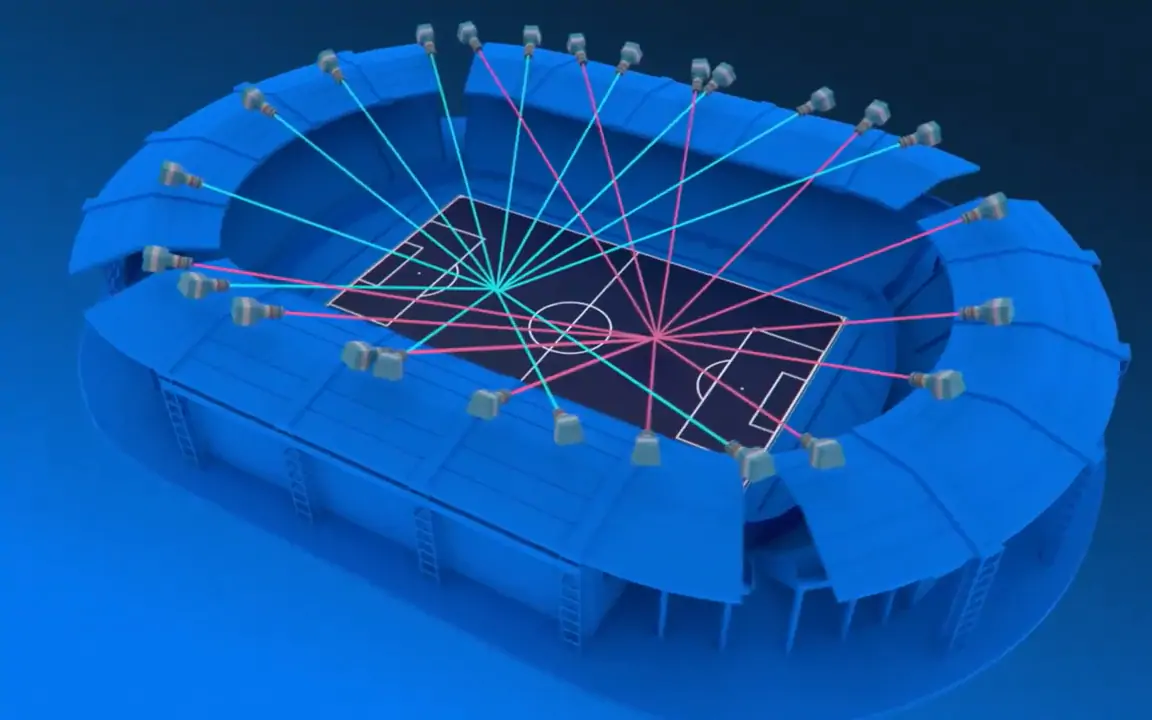
\includegraphics[width=0.7\textwidth]{./images/intelcameras.png}
	\captionsource{High-definiton 5K cameras locations for the Intel True View technology solution in a soccer stadium.\newline}{\cite{intelcameras}}
	\label{fig:intelcameras}
\end{figure}\\
The swiss national soccer team asked to explore state-of-the-art computer vision and visualization technologies for the data of some tv cameras and not to install an expensive system. So what are the possibilities without installing a dozens of high-definition cameras around the stadium to track the bodies of the players. A large related research are has been developed in the last few decades on motion capture technique. 

\section{Motion Capture}
Motion capture tries to track and record the motions of the human body. Whereas the human body is interpreted as a system of rigid links connected by joints as expressed by Xsens \cite{xsens} which is a leading innovator in 3D motion tracking technologies. The developed methods can be divided into different categories, but most technologies do not only benefit from the advantages of one category and combine several techniques to improve the outcome. The main distinction that is particularly relevant for this work is the difference between marker-based motion capture and markerless motion capture \cite{Nogueira2012MotionCF}.

\subsubsection{Marker-Based Motion Capture}
Marker-Based Motion Capture can be further categorized into mechanical, magnetic, acoustic and optical \cite{xsens}. Even the markers are further categorized into active and passive markers. For example passive markers reflect the light back to the cameras in contrast the active markers are equipped with a battery and emit their own light \cite{Nogueira2012MotionCF}.

\begin{itemize}
	\item Mechanical motion system directly track the joints angles using a exoskeleton worn by the person \cite{motionWiki}. This technology is very popular in the film industry. 
	\item Magnetic motion capture systems use the markers as sensors to measure low-frequency magnetic fields generated by a transmitter source. The sensors measure the strength of these magnetic field on order to calculate positions and orientations \cite{magnetic,motionWiki, xsens}. Magnetic systems do not suffer from line of sight problems, thereby the method is useful if the scene is not in the angle of view.
	\item Acoustic tracking systems work with ultrasonic pulses and can compute the position through the time-of-flight of the pulses with triangulation. To work correctly a clear line of sight is needed and to avoid reflections this method should be used outdoors \cite{xsens}.
	\item Optical motion capture uses multiple cameras to track the markers, the markers for this purpose can be passive or active exactly as described above \cite{xsens}. To extract the markers 3D position triangulation is used ad in the acoustic system. There exist even single camera systems but with additionally sensors to measure the lost depth in the image because triangulation is  not possible as noted in \cite{motioncapturetechnologies}.
\end{itemize} 
But in general those approaches are all limited to the fact that the player are required to wear some form of markers on their body. Of course it would be possible to place the markers inside the cloths and shoes but that have to be approved by the FIFA for official games and also by the players themselves. However exactly these technologies are used for video games like the FIFA Football series to capture the movements of the players more realistically.
\begin{figure}[h]
	\centering
	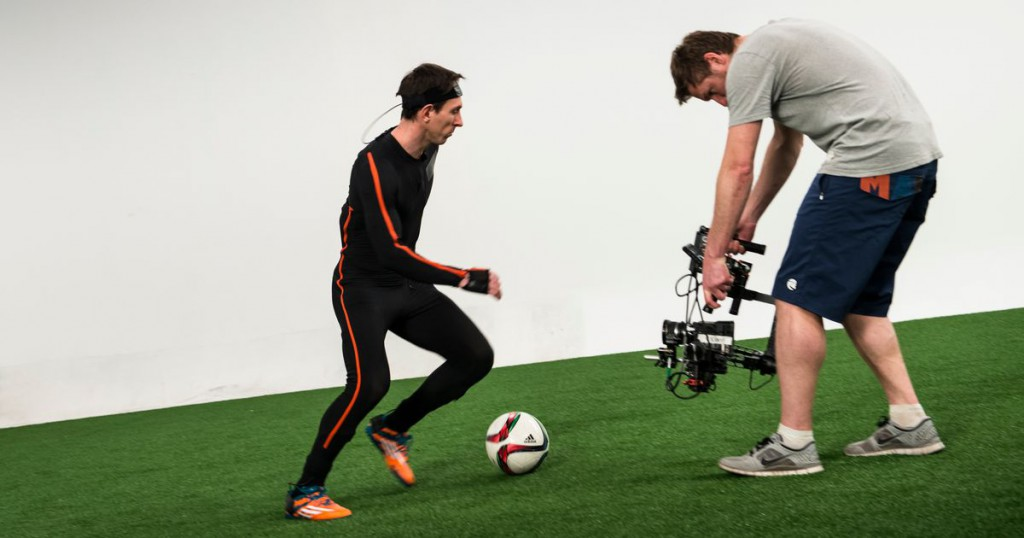
\includegraphics[width=0.7\textwidth]{./images/messi.jpg}
	\captionsource{Messi in Xsens motion capture suit for FIFA 16 to animate his dribbling style as realistically as possible. \newline}{\cite{xsensmessi}}
	\label{fig:messi}
\end{figure}
\subsubsection{Markerless Motion Capture}
Due to the many researches in the field of computer vision, markerless optical motion detection systems are possible. These systems do not rely on a suit with markers which has to be worn, instead they rely on computer vision algorithms to reconstruct the 3D motion from videos and other sensors \cite{motioncapturetechnologies}. 
\begin{figure}[h]
	\centering
	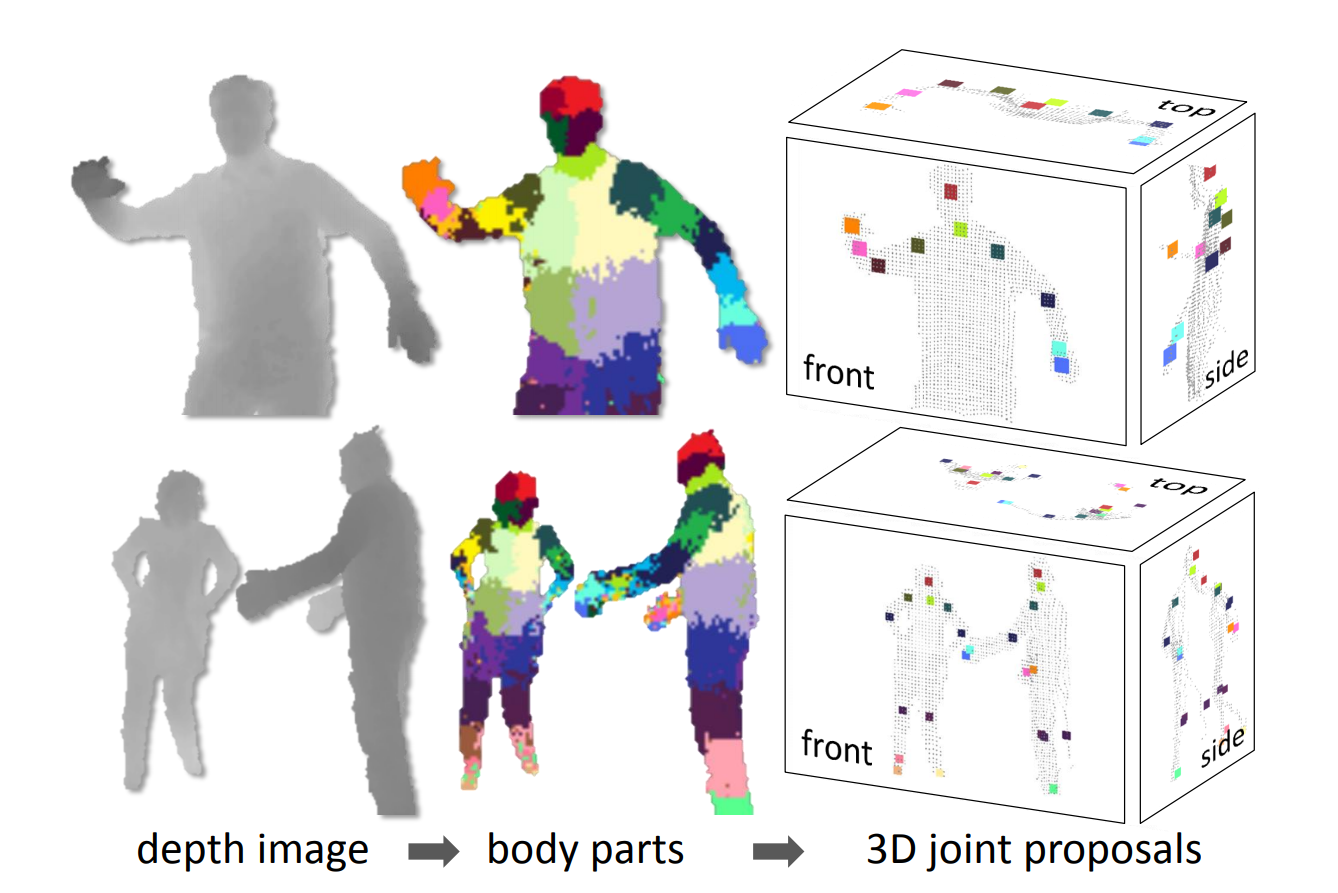
\includegraphics[width=0.7\textwidth]{./images/microsoft.png}
	\captionsource{Overview for the 3D positions reconstruction from one single depth image.\newline}{\cite{microsoft}}
	\label{fig:messi}
\end{figure}
An example for such a system is the Microsoft's Kinect \cite{microsoft}, they localize the 3D positions of body joints from one single depth image. Roughly described they designed an intermediate body parts representation based on an object recognition approach. This presentation consists of several localized body part labels which cover the whole body. This intermediate representation simplifies the difficult pose estimation problem into a simpler classification problem per pixel. But for further reading take a look at the paper \cite{microsoft}.

\section{Human Poses Estimation}
During the last few years the human 2D pose estimation has been greatly improved. Through better object detection algorithms, as the one presented in the section \ref{sec:detectron}, common approaches try to detect a person and run for each detection a single-person pose estimation. The runtime of these so called Top-Down approaches is proportional to the number of detected people in the image \cite{openpose_paper}. To avoid this complexity for multiple people so called buttom-up approaches have been developed as \textit{DeepCut} \cite{deepcut} or \textit{OpenPose} \cite{openpose_paper}. A rough overview how they work is given in the section \ref{sec:openpose} for the \textit{OpenPose} approach. 
\begin{figure}[h]
	\centering
	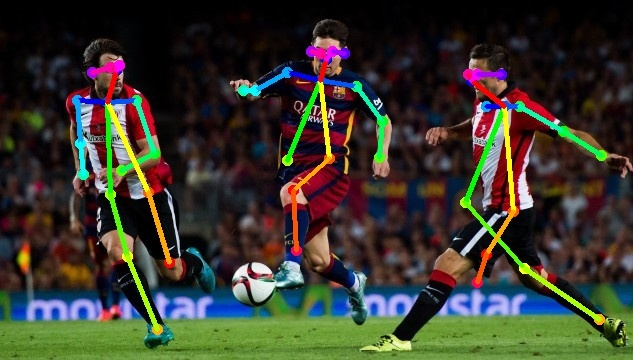
\includegraphics[width=0.7\textwidth]{./images/openpose_example.jpg}
	\captionsource{human 2D pose estimation example with OpenPose\newline}{\cite{openpose_example}}
	\label{fig:openpose_example}
\end{figure}\\
The resulting 2D pose estimation is shown in the figure \ref{fig:openpose_example}. With these technologies we were able to estimate human body joints on two dimensional images which is the beginning for 3D human pose estimations.

In order to understand the 3D geometry the depth is needed but exactly this depth is lost in 2D images. To recover the depth from images or videos there exists already comprehensive work such as \cite{depth_estimation,depth_map}. But these are applied to normal scenes and not explicitly to human bodies. The article \cite{3dpose} describes a method for automatic 3D human pose and shape estimation from a single image. This approach builds upon the 2D joints results of \textit{DeepCut}\cite{deepcut}. Afterwards they fit a statistical body shape model to the 2D joints. The corresponding model is called the \textit{Skinned Multi-Person Linear Model (SMPL)} \cite{smpl} which is a realistic 3D model of the human body learned from thousands of 3D body scans. To fit the model to the 2D joints they minimize an objective function including the error from the projected 3D model joints and the previously estimated 2D joints. In the figure \ref{fig:3dpose_example} an example result from the automatic 3D human pose and shape estimation is presented.
\begin{figure}[h]
	\centering
	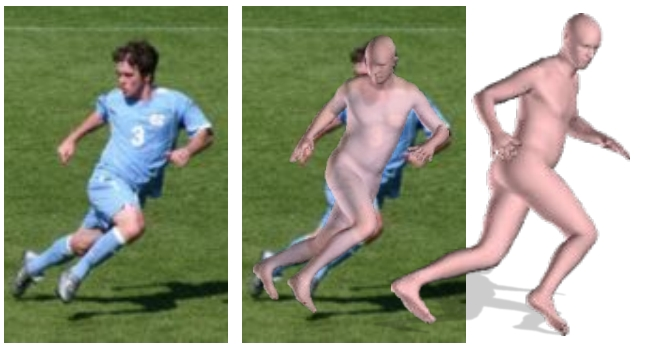
\includegraphics[width=0.7\textwidth]{./images/3dpose_example.jpg}
	\captionsource{To the 2D joints of the original image (not shown) a \textit{SMLP} model is fitted as seen in the middle and on the right side the resulting 3D model is rendered from a different viewpoint. \newline}{\cite{3dpose}}
	\label{fig:3dpose_example}
\end{figure}\\
In contrast to our method they fit a complex statistical body shape model to the 2D joints and end up with a 3D shape model. The three dimensional joint positions are sufficient for our purpose. Additionally we have access to multiple camera views which enables the possibility for triangulation based methods. Along we can benefit from several consecutive frames to not treat each frame individually.


\section{Soccer on Your Tabletop}\label{tabletop}
% general description what they have done
This section presents the main concepts of the project \textit{Soccer on Your Tabletop}\cite{tabletop}. The goal of their work is a moving 3D reconstruction of a soccer game from a single monocular video. The estimation of the depth map of each player represents the core of their work. In the figure \ref{fig:tabletop} a rough overview of their pipeline is given, with the first few steps explained in more detail in the following sections. The reason for the more detailed explanation is their integration in our work which is further outlined in the method chapter.
\begin{figure}[h]
	\centering
	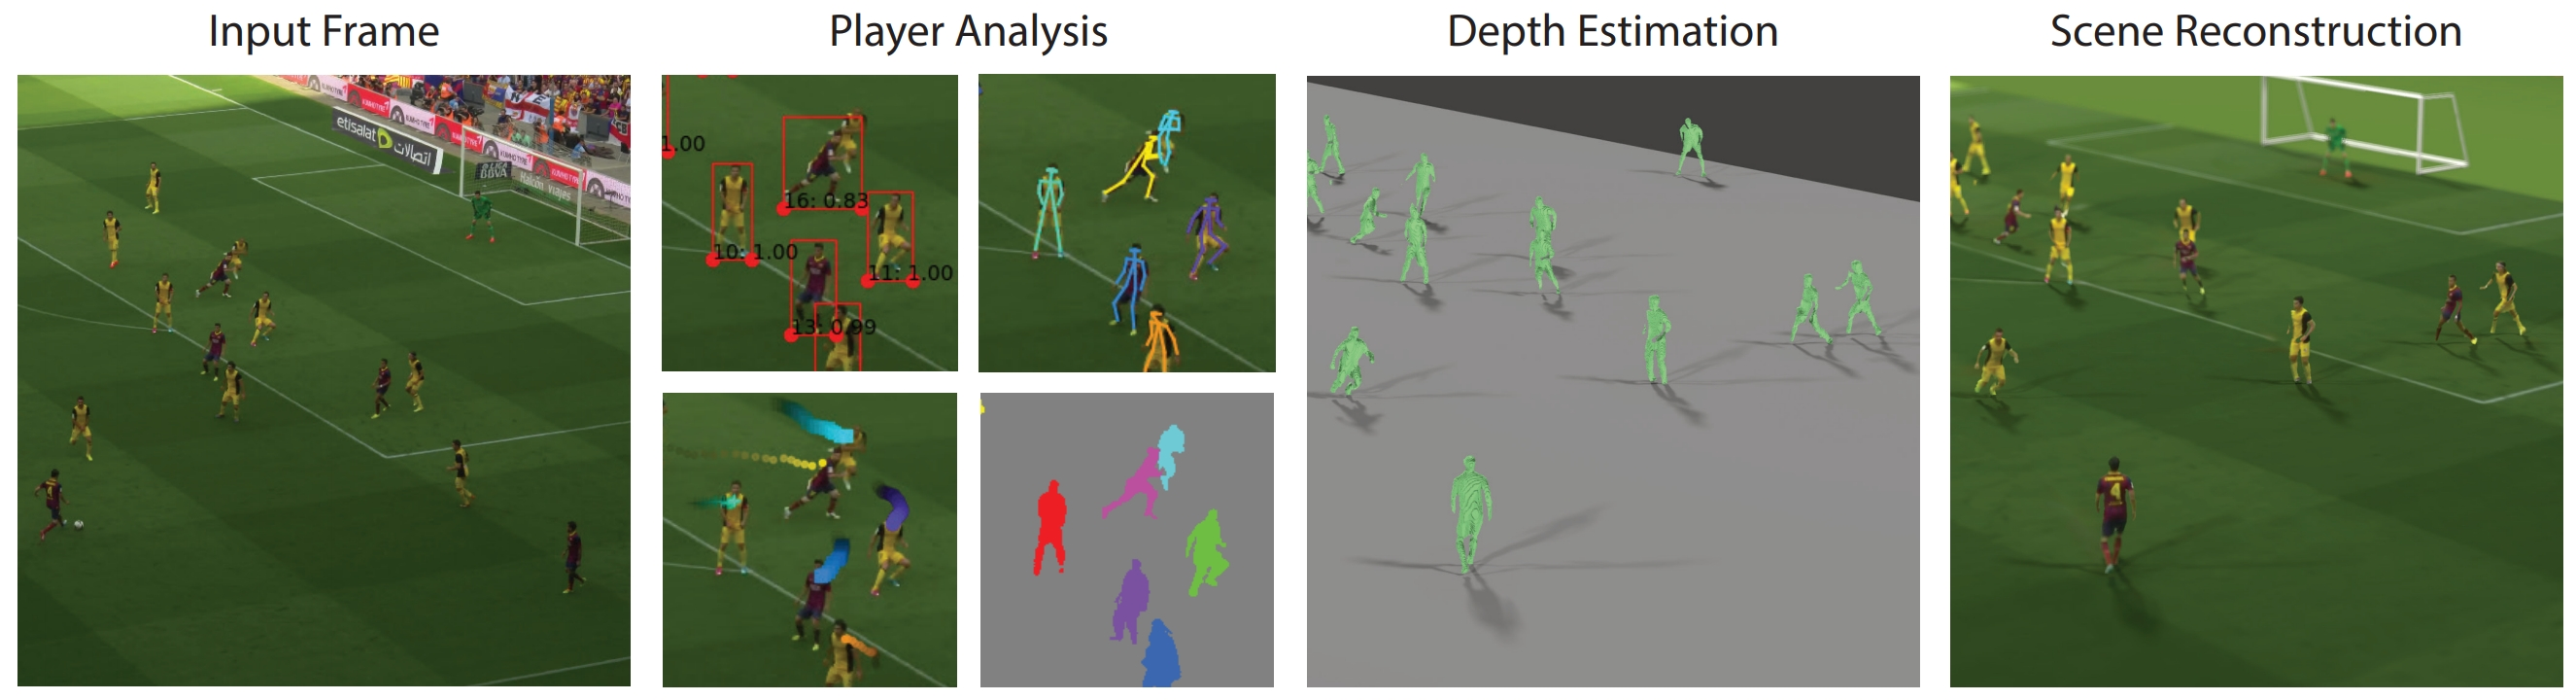
\includegraphics[width=1.\textwidth]{./images/tabletop.jpg}
	\captionsource{Overview of their reconstruction pipeline. In the first step the players from the input frame are analyzed and the camera calibrated. Through the player analysis they segment the player and reconstruct the depth map on the pitch per player. At the end they render the scene in 3D for a complete scene reconstruction. \newline}{\cite{tabletop}}
	\label{fig:tabletop}
\end{figure}

The input are frames from a single monocular video that is being processed. The player analysis consists of several building blocks of existing work. In the first step a state-of-the-art object detection algorithm called \textit{Detectron}\cite{detectron} is used to detect the persons in each frame. The 2D poses for the recognized persons are then determined using \textit{OpenPose}\cite{openpose_paper}. These poses together with the detection are then used to refine the people segmentation \cite{segmentation}. For the per player depth map on the pitch they developed a deep network. The network was trained on video game data, to be more precise they extracted depth maps from EA FIFA games. The advantage of this training data is the specific form in terms of movement, clothing and camera perspective \cite{tabletop}. 

\subsubsection{Building Blocks}
As mentioned above there are multiple building blocks which are also part of our method. For this purpose the theory behind them are further explained in the next few section. How they are integrated into our work is then explained in the method chapter. 


\subsection{Detectron}\label{sec:detectron}
Detectron is a system developed by Facebook AI Research and implements multiple  state-of-the-art object detection algorithms such as Mask R-CNN \cite{r-cnn}, RetinaNet \cite{retinenet} and some others. The system is powered by the Caffe2 deep learning framework which is now part of PyTorch \cite{pytorch}. 

Soccer on your tabletop modified the originally published \textit{infer\_simple.py} file by Detectron which outputs the visualization of the algorithm in PDF format. Instead bounding boxes around the recognized objects and segmentation masks are outputted. At this point in time not only the players but also the spectators and the ball were recognized. In further processing the objects outside of the pitch get removed using the camera calibration and bounding boxes with an area under a specific threshold are removed just to keep the boxes for the players \cite{tabletop}. These are used in later processes. 

\subsection{Calibration}\label{sec:tablecalibration}
During the calibration step, the camera matrix is determined for each frame of a camera. The camera matrix $M$ transforms homogeneous 3D world coordinates to homogeneous 2D image coordinates and can be decomposed into an intrinsic and extrinsic camera matrix. $\mathbf{R}$ and $\mathbf{T}$ build together the extrinsic camera matrix which describes the camera's position and view direction in world coordinates. If you apply the extrinsic matrix to homogeneous 3D world coordinates, they will be transformed by a rotation matrix $\mathbf{R}$ and a translation vector $\mathbf{T}$ to 3D camera coordinates. The intrinsic matrix $\mathbf{A}$ than transforms the 3D camera coordinates to 2D homogeneous screen coordinates. The intrinsic matrix includes the focal length, principal point offsets and the axis skew. The focal length describes the distance between the image plane and the pinhole of the camera. A perpendicular line to the image plane which intersect with the pinhole is called the principal axis. The intersection of the principal axis with the image plane is the principal point and the offsets describe this point with regard to the screen origin. The axis skew is responsible for the shear distortion which is for a true pinhole camera equal to zero \cite{camerablog}.

\subsubsection{Manual Initialization}
The calibration works in two phases, during the first phase four matching pairs of points are selected manually on the first frame and on a 2D reference image of the football field. A matching pair of points consists of the 2D coordinates for the selected point of the first frame and the 3D coordinates for the selected point on the reference image with $z$-coordinates equal to zero. With these point pairs the intrinsic camera matrix $\mathbf{A}$ is determined by a grid search. The grid search estimates for different focal lengths the camera matrices using the \textit{solvePnP} function from the OpenCV library \cite{opencv}. Afterwards the 3D coordinates are projected into the first frame using the previously estimated camera matrices in order to compute a score for the corresponding focal lengths in a least-squares fashion. The result of the grid search are the focal lengths with smallest score and thereby the projection with the smallest error. For the principal point offsets the height and width of the image were simply divided by 2 under the assumption that the principal axis intersects the image at the center. \\
The extrinsic camera matrices are then estimated using the matching pair of points from before with the estimated intrinsic matrix using the \textit{solvePnPRansac} function from the same library. It works in the same fashion as the grid search fo find a solution which minimizes the reprojection error. The use of the \textit{Random sample consensus (RANSAC)}\cite{ransac} scheme, a commonly used iterative method in computer vision which estimates the model parameters using observational data, makes the function robust to outliers \cite{opencv}. 

\subsubsection{Calibration Propagation}
After the manual initialization for the first frame, in the second phase the camera matrices for the next frame are estimated using the matrices from the previous frame. First the edges in the new frame are detected using the canny edge detector \cite{canny}. With the use of the Sobel kernel the image is filtered in order to get the edge gradient and direction for each pixel. Afterwards through non-maximum suppression all pixels are removed which are not the local maximum in the direction of the gradient to consider just pixels which are part of an edge. Hysteresis Thresholding classifies all edges according to two thresholds. Those between the two thresholds are the critical ones and are classified based on their connectivity \cite{canny}. The edges are used to obtain a representation of the image where the pixel values indicate the distance to the nearest background pixel \cite{distance_transform}. By knowing the camera matrices for the last frame, the soccer field is drawn on the image. This in turn is unprojected to obtain a synthetic 3D field. Along with the image with the distance to the nearest background pixel an objective function is defined and minimized to obtain the new camera matrices for the actual frame. The python code is provided by the soccer on your tabletop \cite{tabletop} project.

\subsection{OpenPose}\label{sec:openpose}
Through \textit{Detectron} the location of recognized objects are known but the human 2D poses were needed. To solve this problem the realtime multi-person 2D pose estimation \textit{OpenPose}\cite{openpose_paper} was used. The systems outputs a people array of objects including the poses using the \textit{JSON} file format.

\begin{figure}[h]
	\centering
	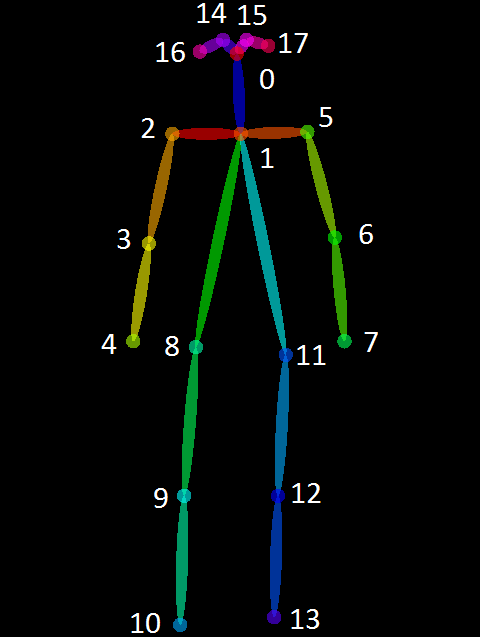
\includegraphics[width=0.4\textwidth]{./images/keypoints_pose_18.png}
	\captionsource{Numbering of the 18 keypoint of the COCO pose format from \textit{OpenPose}. \newline}{\cite{openpose}}
	\label{fig:coco}
\end{figure}
The pose output format (COCO) was used consisting of 18 keypoints as shown in figure \ref{fig:coco}. In addition to the keypoints coordinates the output also includes so called confidence scores per keypoint in the range $[0,1]$ to assess the accuracy.

\subsubsection{Algortihm}
This section is intended to give you a rough understanding of their algorithm as described in their paper \cite{openpose_paper}. Common approaches estimate the poses per person but \textit{OpenPose} follows the bottom-up approach in order to avoid runtime complexity proportional to the number of persons. So the algorithm predicts body part locations independent of the number of persons in the image and tries to connect the individual body parts so that the result are people. This is the reason for the so called buttom-up approach, but in contrast to other methods such as \textit{DeepCut}\cite{deepcut} the final analysis to map the body parts together is more efficient. 
\begin{figure}[h]
	\centering
	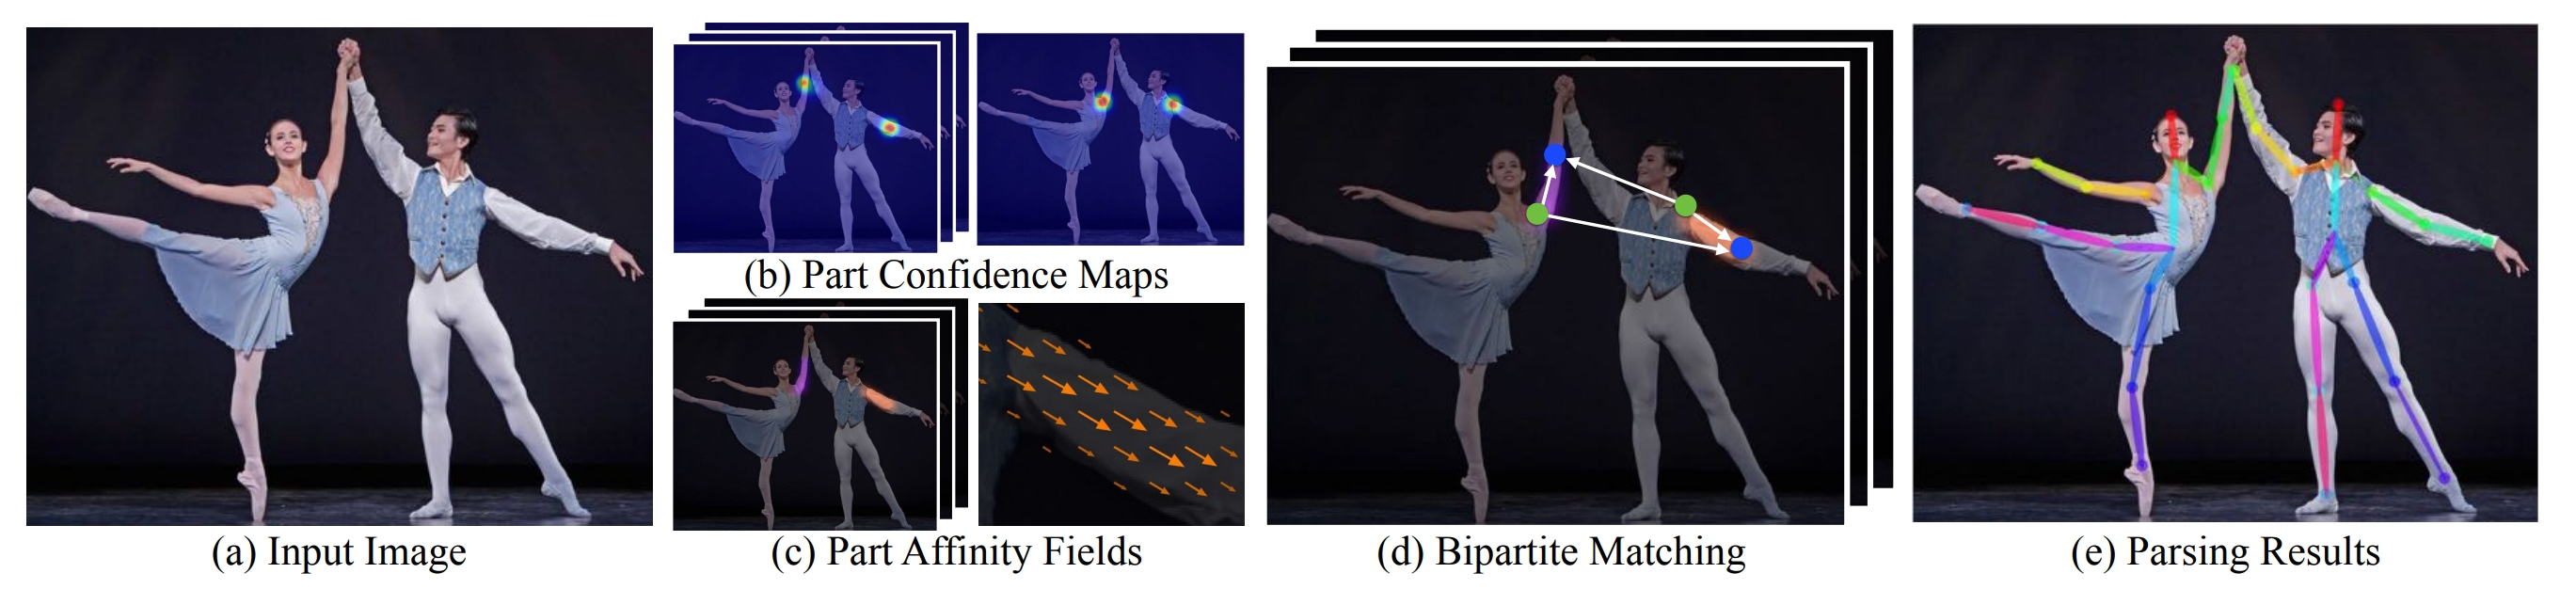
\includegraphics[width=1.\textwidth]{./images/openpose_overview.jpg}
	\captionsource{\textit{OpenPose} Pipeline Overview. The input image (a) is processed to produce the confidence maps (b) and part affinity fields (c) using a CNN. The result is formulated as a bipartite matching problem (d) in order to solve the part association (e).\newline}{\cite{openpose_paper}}
	\label{fig:openpose_overview}
\end{figure}\\
At the begin the input image is processed and analyzed using a convolutional neural network (CNN). The generated feature maps are passed into the first stage which produces a set of part affinity fields (PAFs). A 2D vector in each pixel of every PAF encodes the position and orientation of the limb which is not truly a human limb but a connection of two body parts as shown in figure \ref{fig:openpose_overview} (c). In the following stages the predictions from the previous stage and the original feature are used to refine the estimated PAFs. Afterwards the process is repeated in the same fashion for the body part location to refine the confidence maps. Each body part has its own confidence map which represents the belief for each pixel that this body part is located there as the figure \ref{fig:openpose_overview} (b) shows. So for a single person each confidence map should have one peak for the corresponding location of the body part in the image. These steps in the network differs from other approaches where both the PAFs and the body part locations are refined together but the refinement of the confidence map shows no effect on the PAFs refinement and therefore they are separated which leads to performance improvements and better accuracy. The resulting confidence map for each body part of the network is a collection of all the individual confidence maps for this body part which are combined through non-maxmimum suppression in order to not averaging along the different peaks to be able to distinguish between equal body parts that are close to each other. 
\begin{figure}[h]
	\centering
	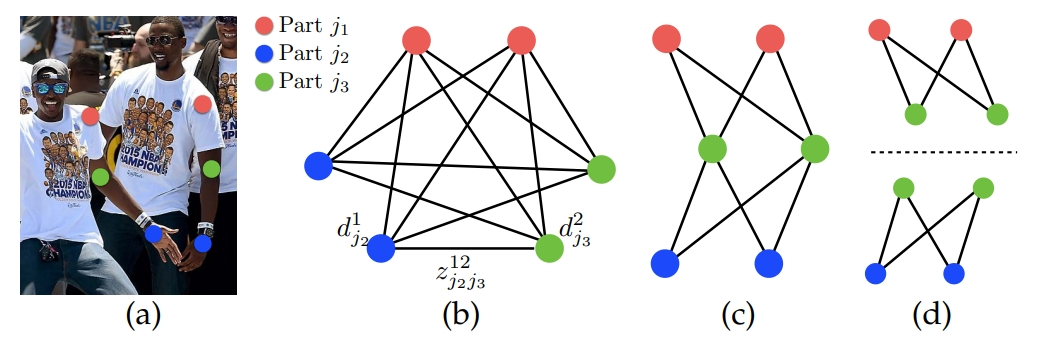
\includegraphics[width=0.8\textwidth]{./images/part_association.jpg}
	\captionsource{\textit{OpenPose's} Part Association formulated as a matching problem with the use of part affinity fields. (a) shows the detected body parts which are then connected in a complete graph (b). The first relaxation reduces the graph to spanning tree skeletons (c) and the second relaxation decompose the graph into bipartit matching subproblems (d).\newline}{\cite{openpose_paper}}
	\label{fig:openpose_mapping}
\end{figure}\\
Given the detected body parts derived from the confidence map for an unknown number of people it is now necessary to map them together to full body poses. For this purpose a confidence score for each pair of the detected body part pairs (candidate limbs) is computed using the line integral on the PAF along the connection between these two parts. Remember the PAFs preserve location and orientation that contribute the additional information needed for this step. So figure \ref{fig:openpose_mapping} (b) shows how each node represents a body part where the color corresponds to the type of body part and the edges expresses these so called candidate limbs weighted by the confidence score. So the part association problem is reformulated as a matching problem which is known to be NP-Hard. But in order to solve the matching problem efficient two relaxations are described. The first relaxation reduces the number of edges to obtain spanning tree skeletons as presented in figure \ref{fig:openpose_mapping} (c), while the second relaxation further decompose the graph into bipartit matching subproblems (d). The matching of these subproblems of adjacent tree nodes can then be determined efficiently and independently. 


\subsection{Depth Map Estimation}
% TODO: eventuell noch depth map estimation erklären wie es gelöst wurde

\section{Filterpy}\label{sec:filterpy}
% some information about the library and the book
FilterPy is a Python library that implements a number of Bayesian filter like for example the Extended Kalman Filter. The author of the library also wrote a book named \textit{Kalman and Bayesian Filter in Python} \cite{filterpybook}. Because the free book was written using Ipython Notebook, it offers the perfect interactive guide to deal with bayesian filter. It starts with some simple filters up to the Kalman filter. It describes the implementation of the library with many examples and explains the mathematical background to understand why it works. For more information visit the the github page \cite{filterpygithub}. 
\chapter{Method}\label{chap:method}
% big overview with a graph
\begin{figure}[h]
	\centering
	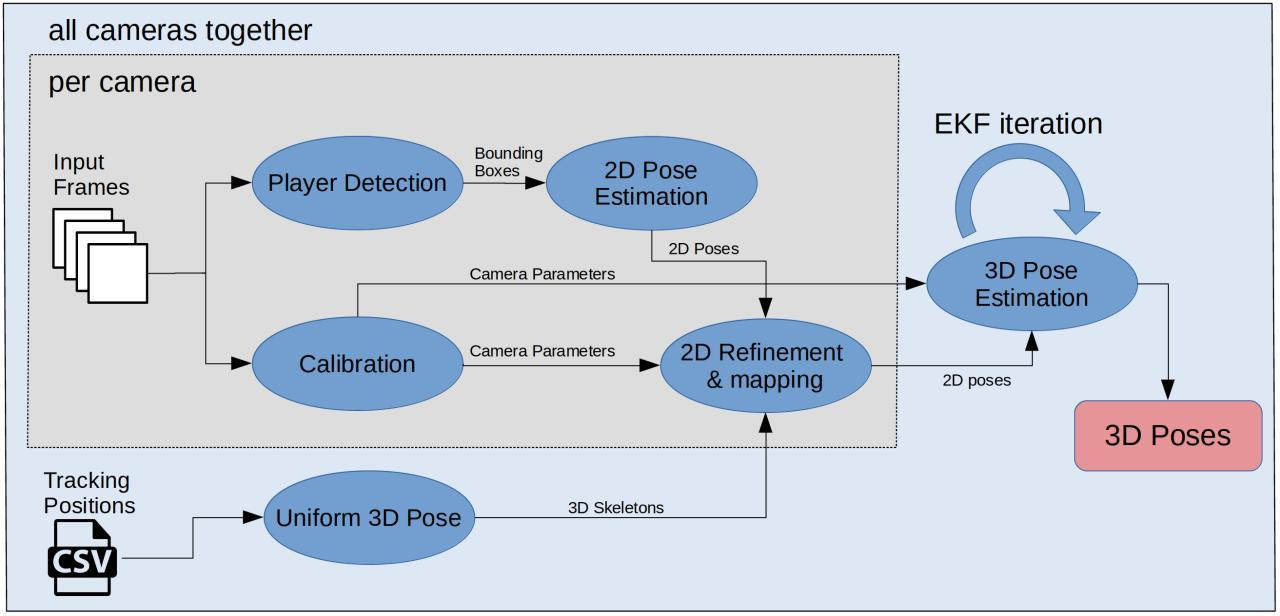
\includegraphics[width=1.0\textwidth]{./images/overview.jpg}
	\caption{Overview of the workflow. Each step gets described in detail during this chapter. The gray area is the process for each camera separately while in the blue area the different cameras are merged.}
	\label{fig:overview}
\end{figure}

\section{Calibration}\label{sec:calibration}
% what is used from soccer on tabletop
%TODO: de Absatz ned ahluege\\

In order to work in three-dimensional space it is required to know how the pixels in a two-dimensional image relate to the three-dimensional world. For the camera model we consider the pinhole camera model for simplicity despite the fact that some cameras suffer from distortion. As mentioned in section \ref{sec:tablecalibration} we were able to calibrate the cameras and got the corresponding camera matrix $M$ which transforms homogeneous 3D world coordinates to homogeneous 2D image coordinates. 

\subsection{Camera Matrix}\label{sec:cameramatrix}
% informations from http://ksimek.github.io/2012/08/14/decompose/

\subsection{Line Detection}
% maybe some details about it

\section{Player Detection}
% details about Detectron

\section{2D Pose Estimation}\label{sec:poseestimation}
% details about openpose

\section{2D Refinement \& mapping}\label{sec:2drefinement}
% details about openpose

\section{3D Pose Fusion}
The next goal is to determine the points in 3D space given its projections onto the multiple images from the different camera perspectives. By knowing the camera matrix of the camera projection from 3D to 2D we know that each point in the image corresponds to a line in 3D space and every point on this line get projected on the same point in the 2D image as mentioned in section \ref{sec:calibration}.

\subsection{Triangulation}
The method to solve this problem is called triangulation. In theory with perfect measurements this method is trivial. So let's assume we got a pair $y_1$ and $y_2$ of corresponding points in two different images. Remember that each point in the image belongs to a line in 3D space which are the green lines in the figure \ref{fig:triangulation}  \cite{triangulation}. The lines intersect at $x$ which is the corresponding point in 3D space. 
\begin{figure}[h]
	\centering
	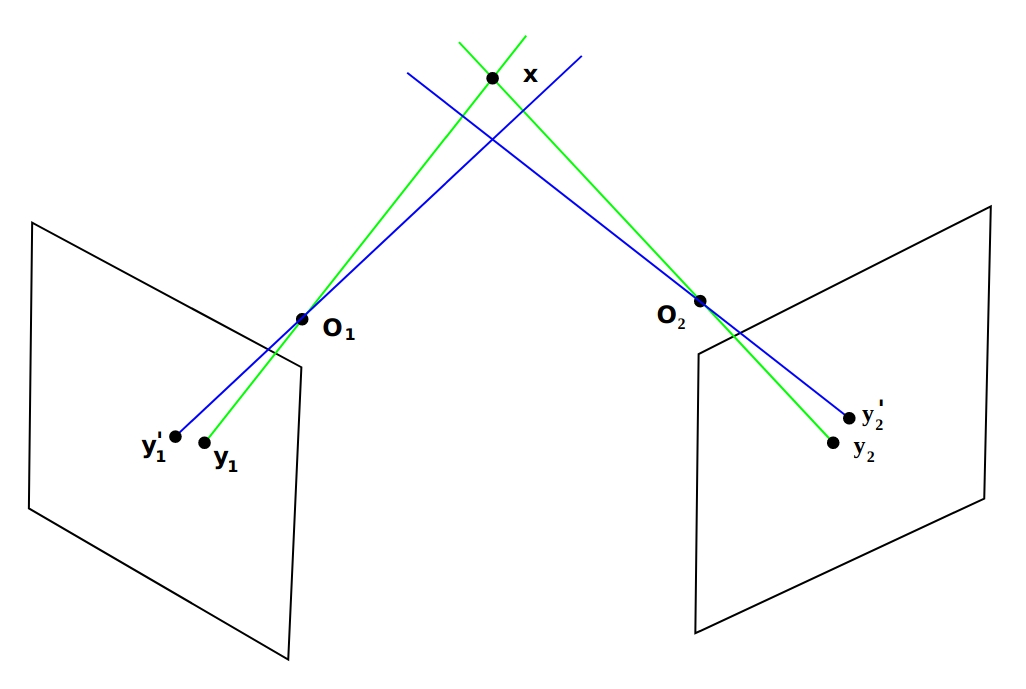
\includegraphics[width=0.7\textwidth]{./images/TriangulationReal.jpg}
	\captionsource{Triangulation visualization of two images with the camera's focal length $O_1$ and $O_2$. The ideal case with perfect measurements in green and the case of measurements with arbitrary accuracy in blue.\newline}{\cite{triangulation}}
	\label{fig:triangulation}
\end{figure}\\
But in practice the the image points are measured with arbitrary accuracy. This leads to the two points $y_1'$ and $y_2'$ in the figure \ref{fig:triangulation}. If you consider the corresponding lines of these two points in 3D space (blue), they must not even intersect and if they do it is not correctly the corresponding 3D point $x$. Reasons for the divergence may be noisy measurements or an inaccurate camera calibration which lead to wrong focal lengths $O_1$ and $O_2$ and therefore to a wrong projection \cite{triangulation}. \\

To find out which 3D point $x'$  is the best estimate for the noisy measurements $y_1'$ and $y_2'$ you usually define an error measurement depending on $x'$ and then minimize this error. Due to the fact that we do not always have all poses in 2D for the triangulation from the different views and the camera calibration is not error-free, I tried to use the Kalman Filter to do the triangulation. By constantly getting new measurements over time and the possibility of predicting the state further in time it seems to be a suitable application to be able to get the 3D poses. 


\subsection{Extended Kalman Filter}\label{sec:EKF}
% details about EKF
The Kalman Filter (KF) is an iterative algorithm, based on the Bayesian Filter, that uses a series of measurements observed over time to find a good state estimation. The filter estimates the state using a form of feedback control where the measured values come into play. The theory in this section is based on the books \textit{An Introduction to the Kalman Filter} \cite{kalmanbook} and \textit{Kalman and Bayesian Filters in Python} \cite{filterpybook}.

\begin{figure}[h]
	\centering
	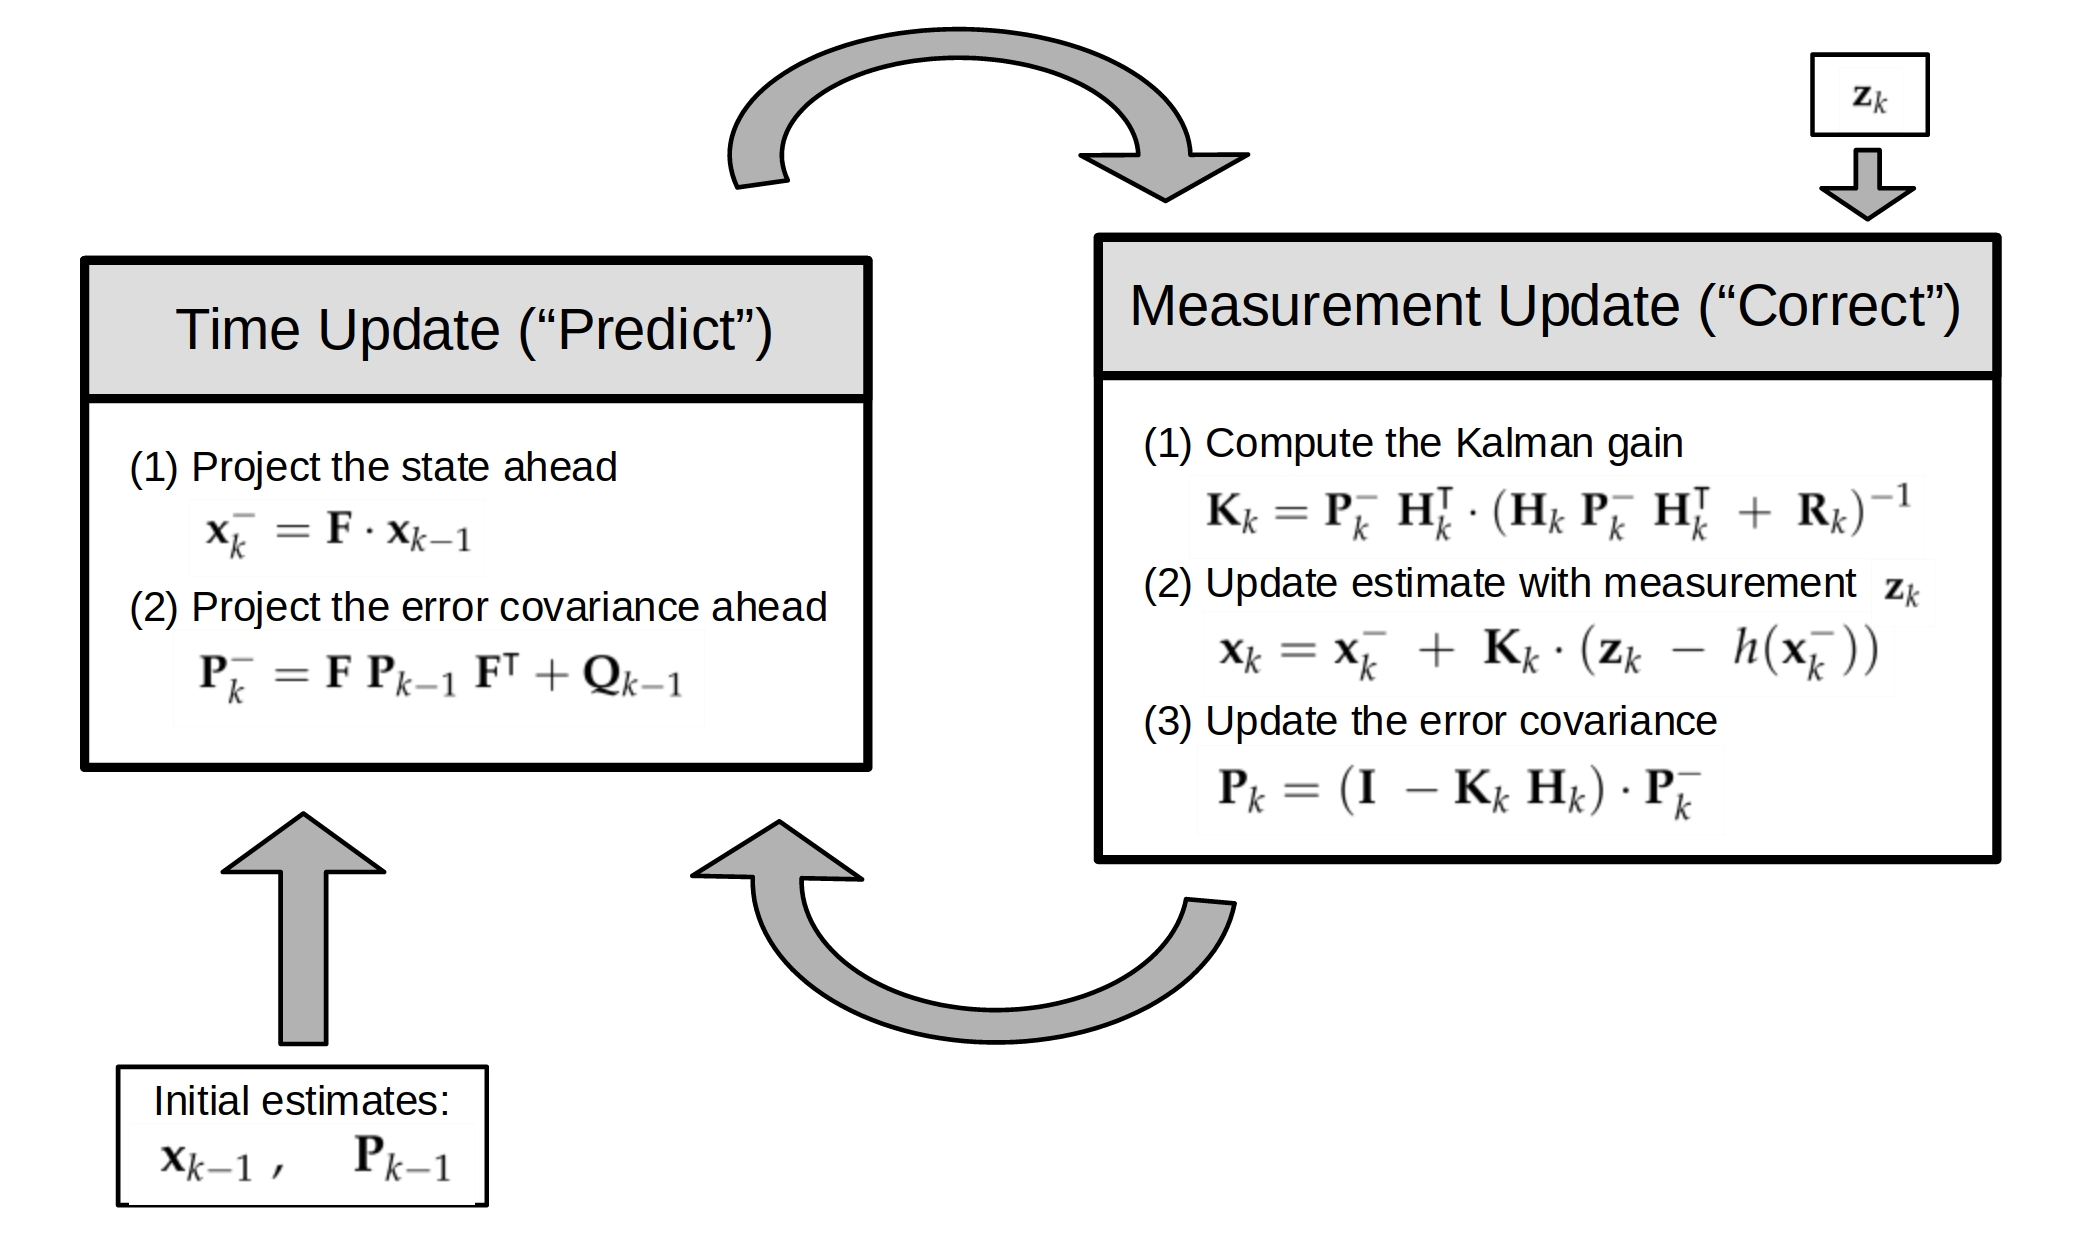
\includegraphics[width=1.0\textwidth]{./images/kalman.jpg}
	\captionsource{Complete picture of the calculations during the two-step process of the Extended Kalman Filter. For the Initialization the values of the first state vector and the error covariance are needed. A new measurement vector is given to the filter for each Measurement Update step.\newline}{Notation slightly adapted from \cite{kalmanbook}}
	\label{fig:kalmanprocess}
\end{figure}
The algorithm works in a two-step process, as shown in figure \ref{fig:kalmanprocess}, which is repeated for every time step or more precise for every frame. In the prediction step, the Kalman Filter projects the current state variable forward in time using the process model and projects the error covariance ahead. In the second step, called the update step, the previously estimated state variable gets updated using the measurement residual weighted with the so called Kalman gain. Additionally the error covariance is updated.
and a new external measurement as described in section x.

In order to update the state variable the residual is needed which is calculated from the current state variable and the newly added measurement $\mathbf{z}_k$. But the state variable is not part of the measurement space, therefore we have to project the state variable to the measurement space. This projection is basically a camera projection and is not linear due to a division, which is the reason why we use the Extended Kalman Filter (EKF). The reason why we work in measurement space and not in state space is because the measurements are not simply invertible which is exactly the goal of the EKF to fuse the 2D measurements into the 3D space.

\subsection{Designing the EKF} 
In the figure \ref{fig:kalmanprocess} and in the following text the notation from the book \textit{An Introduction to the Kalman Filter} \cite{kalmanbook} slightly adapted to the filterpy \cite{filterpybook} notation will be used. We will omit the time subscript $k$ for the definitions of multiple variables in this section for the sake of clarity. For coordinates $x,y,z$ the subscript $w$ is used for the 3D space and $c_k$ for the 2D space of the $k$-th camera. The state and measurement variable $\mathbf{x}, \mathbf{z}$ are written in bold to distinguish from the $x$ and $z$ coordinates. The last note is about the camera matrices which change with every frame. Thus, whenever the camera calibration is mentioned, one always refers to the current calibration.

\subsubsection{State and Measurement}
The EKF is designed to track one person using multiple cameras. The number of cameras is defined in the initialization. As mentioned in section \ref{sec:poseestimation} the OpenPose model \textit{COCO} consists of 15 keypoints. For the $i$-th keypoint the corresponding part of the state vector includes the position in 3D space and their velocities:
\begin{equation}
\mathbf{x}^i \coloneqq 
\begin{bmatrix}
x^i_{w} & y^i_{w} & z^i_{w} & v^i_{x} & v^i_{y} & v^i_{z}\\
\end{bmatrix}^\intercal,   \ \ \forall i \in \{0,1,...,17\}
\end{equation}
All 18 keypoints together form the state vector:
\begin{equation}
\mathbf{x} \coloneqq 
\begin{bmatrix}
\mathbf{x}^0 & \mathbf{x}^1 & \cdots & \mathbf{x}^{17}\\
\end{bmatrix}^\intercal
\end{equation}
The measurement vector $\mathbf{z}$ includes for the $i$-th keypoint the image coordinates $x, y$ for all $n$ cameras:
\begin{equation}
\mathbf{z}^i \coloneqq 
\begin{bmatrix}
x^i_{c_0} & y^i_{c_0} & x^i_{c_1} & y^i_{c_1} & \cdots & x^i_{c_n} & y^i_{c_n}\\
\end{bmatrix}^\intercal, \ \ \forall i \in \{0,1,...,17\}
\end{equation}
The complete measurement vector is again for all 18 keypoints:
\begin{equation}
\mathbf{z} \coloneqq 
\begin{bmatrix}
\mathbf{z}^0 & \mathbf{z}^1 & \cdots & \mathbf{z}^{17}\\
\end{bmatrix}^\intercal
\end{equation}

\subsubsection{Process Model}
For the state propagation $\mathbf{F}$ in the Predict step we use a simple linear model that does not change over time. For the sake of simplicity we assume constant velocity. For several reasons this is not the best choice for modeling the real world. The players move in different directions, the head keypoints behave completely differently to the hand keypoints etc. But due to the high frame rate one can neglect these aspects because the movement from one frame to the next is minimal. The linear motion model for the $x$ coordinates in 3D space is as follows $x = x + v_x\cdot \Delta t$. The time step $\Delta t$ represents the time between two frames. The resulting state transition model $F'$ propagates the state vector for the $i$-th keypoint $x^i$ further in time,
\begin{equation}
\mathbf{F}^i \coloneqq 
\begin{bmatrix}
1 & 0 & 0 & \Delta t & 0 & 0 \\
0 & 1 & 0 & 0 & \Delta t & 0 \\
0 & 0 & 1 & 0 & 0 & \Delta t \\
0 & 0 & 0 & 1 & 0 & 0 \\
0 & 0 & 0 & 0 & 1 & 0 \\
0 & 0 & 0 & 0 & 0 & 1 \\
\end{bmatrix}, \ \ \forall i \in \{0,...,17\}
\end{equation}
so the resulting complete state propagation matrix $\mathbf{F}$ is a diagional matrix expressed using multiple submatrices $\mathbf{F}^i$:
\begin{equation}
\mathbf{F} \coloneqq 
\begin{bmatrix}
\mathbf{F}^1 & & \\
& \ddots & \\
& & \mathbf{F}^{17}
\end{bmatrix}
\end{equation}
This results in the first equation of the extended Kalman filter to project the state ahead:
\begin{equation}\label{eq:state}
\mathbf{x}_k^- = \mathbf{F} \cdot \mathbf{x}_{k-1}
\end{equation}

Together with the next equation \ref{eq:covariance}, those two form the prediction step of the EKF. The estimation error covariance $\mathbf{P}$ gets projected  from the previous time step $k-1$ to the current time step $k$.
\begin{equation}\label{eq:covariance}
\mathbf{P}_k^- = \mathbf{F}\ \mathbf{P}_{k-1}\ \mathbf{F}^\intercal + \mathbf{Q}_{k-1}
\end{equation}
At the begin the covariance matrix $\mathbf{P}$ have to be initialized and afterwards the filter takes care of updating its value. We know that the position and velocity are correlated but due to the fact that we use constant velocity in our model we just initialize $\mathbf{P}$ to zero. The matrix is a square matrix of the same dimension as the state vector. 

\subsubsection{Noise}
In both equation \ref{eq:covariance} and \ref{eq:covariance2} we add a covariance matrix derived from white Gaussian noise. $\mathbf{Q}$ is a square matrix of the same dimension as the state vector $\mathbf{x}_k$ and is called the process noise covariance. The matrix $\mathbf{R}$ is also a square matrix with the dimension of the measurement vector $\mathbf{z}_k$ and is called the measurement noise covariance. They're called white Gaussian noise because they are independent of each other with normal probability distribution. During the EKF iteration they stay constant with values $\sigma_q = 0.3$ and $\sigma_r = 0.02$:
\begin{equation}
	\mathbf{Q} \coloneqq 
	\begin{bmatrix}
	\sigma_q & & \\
	& \ddots & \\
	& & \sigma_q
	\end{bmatrix}
\ \qquad \qquad \qquad \qquad 
\mathbf{R} \coloneqq 
\begin{bmatrix}
\sigma_r & & \\
& \ddots & \\
& & \sigma_r
\end{bmatrix}
\end{equation}
The reason for the higher process noise is the inaccurate process model with constant velocity. So the filter tries to rely more on the measurements than on the prediction as desired.


\subsubsection{Kalman gain and Error covariance}
The residual gets added to the predicted state variable $\mathbf{x}_k^-$ as described in the next section. But the residual is weighted by the Kalman gain. Higher values for the Kalman gain indicate that we give more trust to the measurement and a lower values indicate that we rely more on the prediction. So if the measurement uncertainty $\mathbf{R}_k$ is smaller with respect to the error covariance $\mathbf{P}_k^-$ we rely more on the measurement. The computation for the Kalman gain takes place in the Measurement Update step: 
\begin{equation}
\mathbf{K}_k = \mathbf{P}_k^-\ \mathbf{H}_k^\intercal\cdot (\mathbf{H}_k\ \mathbf{P}_k^-\ \mathbf{H}_k^\intercal \ + \ \mathbf{R}_k)^{-1}
\end{equation}
Another equation in the Measurement Update step is the update of the error covariance $\mathbf{P}_k$. 
\begin{equation}\label{eq:covariance2}
\mathbf{P}_k = (\mathbf{I} \ - \mathbf{K}_k\ \mathbf{H}_k)\cdot \mathbf{P}_k^-
\end{equation}
In contrast to $\mathbf{Q}$ and $\mathbf{R}$ which are both constant, the error covariance $\mathbf{P}_k$ and the Kalman gain $\mathbf{K}_k$ will stabilize quickly and then remain constant as described in \cite{kalmanbook}.
These two equations involves the matrix $\mathbf{H}$ which is explained in the section \ref{sec:jacobian} below.

\subsubsection{Measurement Model}
The measurement model is designed through a function $h$ which is responsible to relate the state vector $\mathbf{x}_k$ to the measurement $\mathbf{z}_k$. As we mentioned in section \ref{sec:EKF} this function projects the state variable into the measurement space in order to be able to compute the residual which leads to this equation for the Measurement Update step:
\begin{equation}
\mathbf{x}_k = \mathbf{x}_k^- \ + \ \mathbf{K}_k\cdot (\mathbf{z}_k \ - \ h(\mathbf{x}_k^-))
\end{equation}
The explanation how the function $h$ looks like and what the related matrix $\mathbf{H}_x$ is will follow in detail. The filterpy implementation \cite{filterpydoc} of the EKF requires for the update step the function $h$ with the arguments $\mathbf{x}_k$ and the camera matrices for all cameras. The output of this function is a vector which looks exactly like the measurement vector $\mathbf{z}_k$ but do not get confused, it is just the same space and no new measurement vector:
\begin{equation}
h(\mathbf{x}^-_k, \text{camera matrices}) = \mathbf{z}_{transformed}
\end{equation}

As mentioned in section \ref{sec:cameramatrix} a homogeneous point in the 3D space can be projected to the image screen using the camera matrix $\mathbf{M}$. I will explain this step for the $x_w,y_w,z_w$ coordinates of the state vector $\mathbf{x}_k$ for one keypoint to map to the corresponding measurement space of one specific camera $j$. I will omit the time subscript $k$ in this section for the sake of understanding. 
\begin{align} 
\mathbf{M}_{c_j} \cdot 
\begin{bmatrix}
x_w \\
y_w \\
z_w \\
1 \\
\end{bmatrix} &= 
\mathbf{A}_{c_j} \begin{bmatrix}
\mathbf{R}_{c_j}&|&\mathbf{T}_{c_j} \\
\end{bmatrix}
\begin{bmatrix}
x_w \\
y_w \\
z_w \\
1 \\
\end{bmatrix} \\
& = 
\begin{bmatrix}
f_x & 0 & x_0 \\
0 & f_y & y_0 \\
0 & 0 & 1\\
\end{bmatrix} 
\begin{bmatrix}
r_{1,1} & r_{1,2} & r_{1,3}& t_x \\
r_{2,1} & r_{2,2} & r_{2,3}& t_y \\
r_{3,1} & r_{3,2} & r_{3,3}& t_z \\
\end{bmatrix}
\begin{bmatrix}
x_w \\
y_w \\
z_w \\
1 \\
\end{bmatrix} \\
& = 
\begin{bmatrix}\label{eq:homogenous}
x_{c_j}' \\
y_{c_j}' \\
z_{c_j}' \\
\end{bmatrix}
\end{align}
In order to get the correct scale and dimension for the screen coordinates  $x_{c_j}, y_{c_j}$ one have to divide the result from equation \ref{eq:homogenous} by $z_{c_j}$ and drop the last entry for the $z$ coordinate. This forms a part of the function $h$:
\begin{align}\label{eq:screencoordinates}
\hat{h}(\begin{bmatrix}
x_w \\
y_w \\
z_w \\
\end{bmatrix},\  \mathbf{A}_{c_j}, \mathbf{R}_{c_j}, \mathbf{T}_{c_j}) &=
\begin{bmatrix}
	x_{c_j} \\
	y_{c_j} \\
\end{bmatrix} \\
&= 
\begin{bmatrix}
\frac{x_{c_j}'}{z_{c_j}'} \\
\frac{y_{c_j}'}{z_{c_j}'} \\
\end{bmatrix} = 
\begin{bmatrix}
\frac{f_x \cdot (r_{1,1} \cdot x_w + r_{1,2} \cdot y_w + r_{1,3} \cdot z_w + t_x)}{r_{3,1} \cdot x_w + r_{3,2} \cdot y_w + r_{3,3} \cdot z_w + t_z } + x_0 \\
\frac{f_y \cdot (r_{2,1} \cdot x_w + r_{2,2} \cdot y_w + r_{2,3} \cdot z_w + t_x)}{r_{3,1} \cdot x_w + r_{3,2} \cdot y_w + r_{3,3} \cdot z_w + t_z } + y_0 \\
\end{bmatrix}
\end{align}
To make it clear once again, this was just to transform the 3D coordinates for one keypoint into the image space of one camera. So for the $i$-th keypoint of the state vector $\mathbf{x}_k$ we drop the velocities and transform the 3D coordinates to screen coordinates for each of the $n$ cameras. This gives us a bigger part of $h$:
\begin{align}
h_i(\begin{bmatrix}
x^i_w \\
y^i_w \\
z^i_w \\
\end{bmatrix},\ \text{camera matrices}) 
& = 
\begin{bmatrix}
\hat{h}(
\begin{bmatrix}
x^i_w \\
y^i_w \\
z^i_w \\
\end{bmatrix},\  \mathbf{A}_{c_0}, \mathbf{R}_{c_0}, \mathbf{T}_{c_0})\\
\vdots \\
\hat{h}(
\begin{bmatrix}
x^i_w \\
y^i_w \\
z^i_w \\
\end{bmatrix},\  \mathbf{A}_{c_n}, \mathbf{R}_{c_n}, \mathbf{T}_{c_n})
\end{bmatrix}
\end{align}
Finally we can formulate the whole function $h$ for all 18 keypoints:
\begin{align}
h(\mathbf{x}^-_k, \text{camera matrices}) 
&= 
\begin{bmatrix}
h_0(\begin{bmatrix}
x^0_w \\
y^0_w \\
z^0_w \\
\end{bmatrix},\ \text{camera matrices})\\
\vdots \\
h_{17}(\begin{bmatrix}
x^{17}_w \\
y^{17}_w \\
z^{17}_w \\
\end{bmatrix},\ \text{camera matrices}) 
\end{bmatrix}\\
&= \mathbf{z}_{transformed}
\end{align}

\subsubsection{Jacobian Matrix H} \label{sec:jacobian}
By the fact that the relationship between state space and the measurement space is a nonlinear function $h$ we need to linearize it by evaluating its partial derivatives with respect to the state vector $\mathbf{x}_k$ like a Taylor series. The resulting matrix is the Jacobian matrix $\mathbf{H}_k$. How the derivations of one screen coordinate pair (the $i$-th keypoint) like in equation \ref{eq:screencoordinates} for the camera $j$ looks like is explained as follows:
\begin{equation}\label{eq:partial}
\mathbf{H}_{c_j}^i = 
\begin{bmatrix}
\frac{\partial x^i_{c_j}}{\partial x^i_w} & \frac{\partial x^i_{c_j}}{\partial y^i_w} & \frac{\partial x^i_{c_j}}{\partial z^i_w} & \frac{\partial x^i_{c_j}}{\partial v^i_x} & \frac{\partial x^i_{c_j}}{\partial v^i_y} & \frac{\partial x^i_{c_j}}{\partial v^i_z} \\
\frac{\partial y^i_{c_j}}{\partial x^i_w} & \frac{\partial y^i_{c_j}}{\partial y^i_w} & \frac{\partial y^i_{c_j}}{\partial z^i_w} & \frac{\partial y^i_{c_j}}{\partial v^i_x} & \frac{\partial y^i_{c_j}}{\partial v^i_y} & \frac{\partial y^i_{c_j}}{\partial v^i_z} \\
\end{bmatrix}
\end{equation}
The matrix $\mathbf{H}_{c_j}^i$ would be much wider because of the partial derivatives for the other state variables but they are all zero so we just note this block matrix and build the Jacobian $\mathbf{H}$ with multiple similar blocks. So the whole corresponding block of the Jacobian for the $i$-th keypoint with respect to all $n$ cameras is presented:
\begin{equation}
\mathbf{H}^i =
\begin{bmatrix}
\mathbf{H}_{c_0}^i \\
\mathbf{H}_{c_1}^i \\
\vdots \\
\mathbf{H}_{c_n}^i \\
\end{bmatrix}
\end{equation}
And finally we can formulate the entire Jacobian $\mathbf{H}_k$ with the partial derivatives for the entire state vector, note that in the steps above the subscript $k$ has been removed for readability.
\begin{equation}
\mathbf{H}_k =
\begin{bmatrix}
\mathbf{H}^0 &  & \\
& \ddots & \\
& & \mathbf{H}^{17}
\end{bmatrix}
\end{equation}
Like the function $h$ the filterpy \cite{filterpydoc} implementation also requires the Jacobian of $h$ as input for the update step. So the Jacobian $\mathbf{H}_x$ is also a function with the same arguments as the function $h$, namely the state vector $\mathbf{x}_k$ and the camera matrices. For the readability we first define some variables which are used afterwards:
\begin{align}
r_{1}\mathbf{x}^i \coloneqq r_{1,1} \cdot x_w^i + r_{1,2} \cdot y_w^i + r_{1,3} \cdot z_w^i \\
r_{2}\mathbf{x}^i \coloneqq r_{2,1} \cdot x_w^i + r_{2,2} \cdot y_w^i + r_{2,3} \cdot z_w^i \\
r_{3}\mathbf{x}^i \coloneqq r_{3,1} \cdot x_w^i + r_{3,2} \cdot y_w^i + r_{3,3} \cdot z_w^i
\end{align}
So what's left are the partial derivatives. The computation for those from equation \ref{eq:partial} are shown with respect to the $i$-th keypoint and the $j$-th camera, the others are analog but with the corresponding keypoint coordinates and the corresponding camera matrices.
\begin{align}
\frac{\partial x^i_{c_j}}{\partial x^i_w} = \frac{f_x \cdot r_{1,1}}{r_{3}\mathbf{x}^i + t_z} - \frac{f_x \cdot r_{3,1}(r_{1}\mathbf{x}^i + t_x)}{(r_{3}\mathbf{x} + t_z)^2}\\
\frac{\partial x^i_{c_j}}{\partial y^i_w} = \frac{f_x \cdot r_{1,2}}{r_{3}\mathbf{x}^i + t_z} - \frac{f_x \cdot r_{3,2}(r_{1}\mathbf{x}^i + t_x)}{(r_{3}\mathbf{x} + t_z)^2}\\
\frac{\partial x^i_{c_j}}{\partial z^i_w} = \frac{f_x \cdot r_{1,3}}{r_{3}\mathbf{x}^i + t_z} - \frac{f_x \cdot r_{3,3}(r_{1}\mathbf{x}^i + t_x)}{(r_{3}\mathbf{x} + t_z)^2}\\
\frac{\partial y^i_{c_j}}{\partial x^i_w} = \frac{f_y \cdot r_{2,1}}{r_{3}\mathbf{x}^i + t_z} - \frac{f_y \cdot r_{3,1}(r_{2}\mathbf{x}^i + t_y)}{(r_{3}\mathbf{x} + t_z)^2}\\
\frac{\partial y^i_{c_j}}{\partial y^i_w} = \frac{f_y \cdot r_{2,2}}{r_{3}\mathbf{x}^i + t_z} - \frac{f_y \cdot r_{3,2}(r_{2}\mathbf{x}^i + t_y)}{(r_{3}\mathbf{x} + t_z)^2}\\
\frac{\partial y^i_{c_j}}{\partial z^i_w} = \frac{f_y \cdot r_{2,3}}{r_{3}\mathbf{x}^i + t_z} - \frac{f_y \cdot r_{3,3}(r_{2}\mathbf{x}^i + t_y)}{(r_{3}\mathbf{x} + t_z)^2}\\ \frac{\partial x^i_{c_j}}{\partial v^i_x} = \frac{\partial x^i_{c_j}}{\partial v^i_y} = \frac{\partial x^i_{c_j}}{\partial v^i_z} = \frac{\partial y^i_{c_j}}{\partial v^i_x} = \frac{\partial y^i_{c_j}}{\partial v^i_y} = \frac{\partial y^i_{c_j}}{\partial v^i_z} = 0
\end{align}

\subsubsection{State Initialization}
% TODO: How is the state initialized at the begin
TODO

All together result in the final EKF. For a good overview the five equations for the filter are repeated here:

\textbf{The Update ("Predict"):}

(1) Projet the state ahead:
\begin{equation}
\mathbf{x}_k^- = \mathbf{F} \cdot \mathbf{x}_{k-1}
\end{equation}
(2) Project the error covariance ahead:
\begin{equation}
\mathbf{P}_k^- = \mathbf{F}\ \mathbf{P}_{k-1}\ \mathbf{F}^\intercal + \mathbf{Q}_{k-1}
\end{equation}
\textbf{Measurement Update ("Correct"):}

(1) Compute the Kalman gain:
\begin{equation}
\mathbf{K}_k = \mathbf{P}_k^-\ \mathbf{H}_k^\intercal\cdot (\mathbf{H}_k\ \mathbf{P}_k^-\ \mathbf{H}_k^\intercal \ + \ \mathbf{R}_k)^{-1} 
\end{equation}
(2) Update estimate with measurement $\mathbf{z}_k$:
\begin{equation}
\mathbf{x}_k = \mathbf{x}_k^- \ + \ \mathbf{K}_k\cdot (\mathbf{z}_k \ - \ h(\mathbf{x}_k^-))
\end{equation} 
(3) Update the error covariance:
\begin{equation}
\mathbf{P}_k = (\mathbf{I} \ - \mathbf{K}_k\ \mathbf{H}_k)\cdot \mathbf{P}_k^-
\end{equation}

\chapter{Results and Discussion}\label{chap:results}


\chapter{Conclusion}\label{chap:conclusion}
% summarize again what your paper did, but now emphasize more the results, and comparisons

% write conclusions that can be drawn from the results found and the discussion presented in the paper

\section{Future Work}


\appendix

\chapter{Dummy Appendix}

You can defer lengthy calculations that would otherwise only interrupt
the flow of your thesis to an appendix.


\backmatter

\bibliographystyle{plain}
\bibliography{refs}

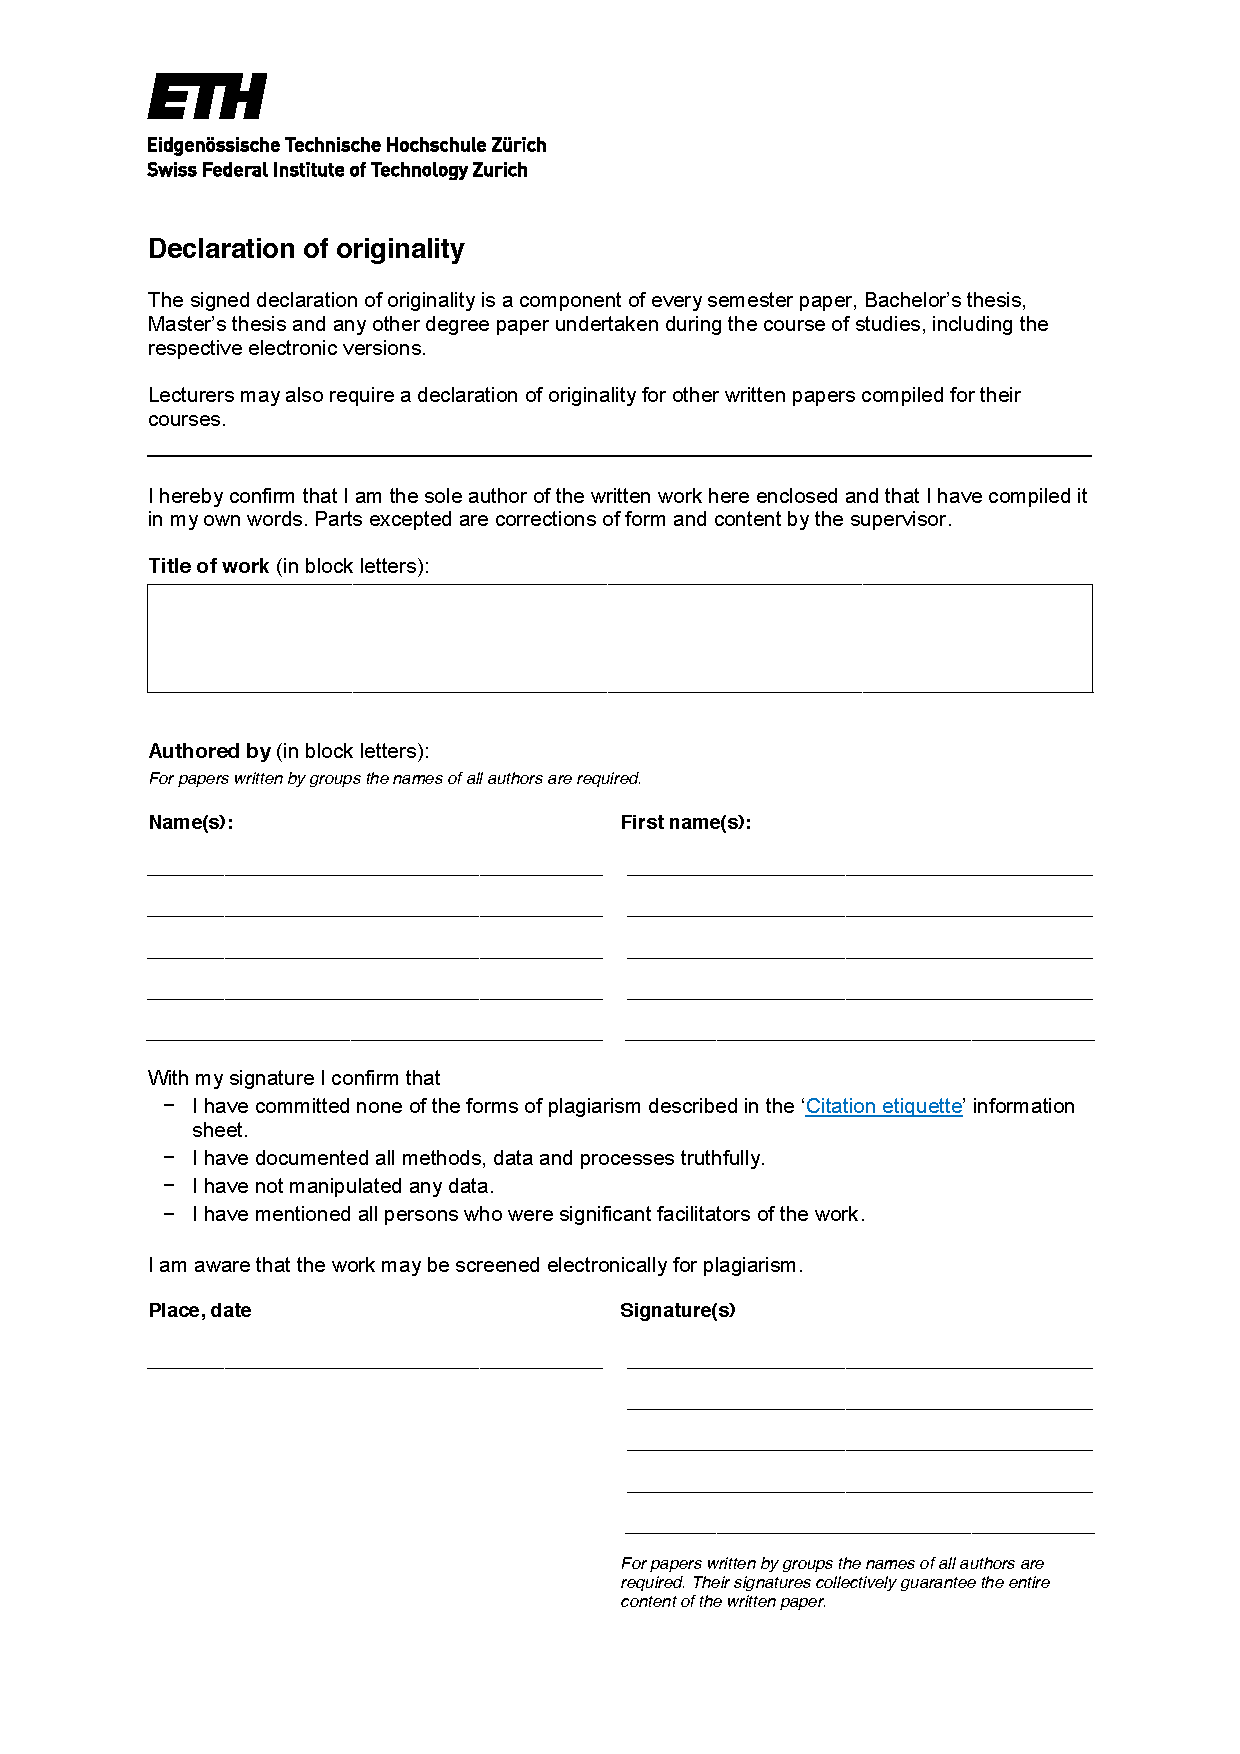
\includepdf[pages={-}]{declaration-originality.pdf}

\end{document}
